\documentclass{astroedu-lab}

\begin{document}

\pagestyle{plain}

\begin{problem}{\huge Лабораторная работа 3.2.6\\\\Исследование гальванометра\\\\Выполнил Жданов Елисей Б01-205}

\section{Цель работы:}

Изучение работы высокочувствительного зеркального гальванометра магнитоэлектрической системы в режимах измерения постоянного тока и электрического заряда.

\section{Оборудование:}

зеркальный гальванометр с осветителем и
	шкалой, источник постоянного напряжения, делитель напряжения, магазин сопротивлений, эталонный конденсатор, вольтметр, переключатель, ключи, линейка.
	

\section{Теоретическая справка}

Баллистическим гальванометром называют электроизмерительный прибор магнитоэлектрической системы, отличающийся высокой чувствительностью к току и сравнительно большим периодом колебаний подвижной системы (рамки).

Рис. 1. Рамка с током в магнитном поле
Главной частью баллистического гальванометра является подвешенная на вертикальной нити рамка, помещённая в поле постоянного магнита. Вырез цилиндрической формы в полюсах магнита и ферромагнитный цилиндр на оси системы делают поле в зазоре радиальным (рис. 1). Скреплённое с рамкой зеркальце служит для измерения угла поворота рамки. К рамке прикреплён полый цилиндр, который сильно увеличивает момент инерции и, следовательно, период колебаний подвижной системы, не очень её утяжеляя. Магнит и подвижная система заключены в защитный кожух. В баллистических гальванометрах применяют сильные постоянные магниты и рамки с большим количеством витков, подвешенные на тонких нитях с малой упругостью.

Баллистический гальванометр позволяет измерять как постоянный ток (стационарный режим), так и заряд, протекший через рамку за некоторое время (баллистический режим). В баллистическом режиме гальванометр может работать, если время протекания заряда много меньше периода собственньх колебаний подвижной рамки. Поэтому период колебаний рамки делают большим (5-15 с). Это время учитывает реакцию экспериментатора, которому надо успеть сделать отсчёт максимального отклонения рамки.

\begin{figure}[!h]
	\centering
	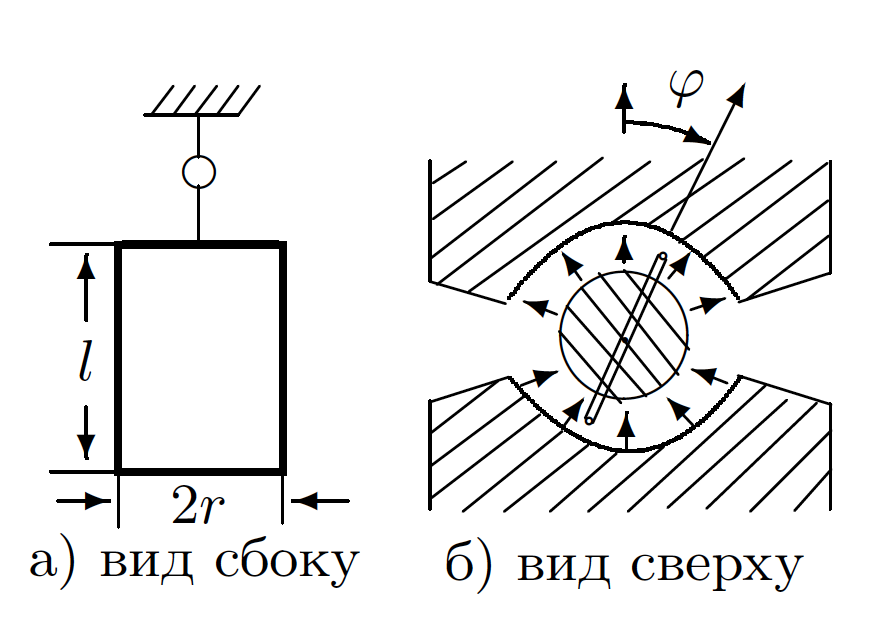
\includegraphics[width=0.5\textwidth]{ramka.png}
	\label{fig:boiler}
\end{figure}

\subsection{Уравнение движения рамки в магнитном поле}

На помещённую в магнитное поле рамку гальванометра, по которой течёт ток, действуют момент сил закрученной нити, момент сил трения (сопротивление воздуха и т. п.) и момент магнитньх сил (сил Ампера). Последний можно условно разделить на две составляющие: момент, действующий на составляющую тока, обусловленную ЭДС внешней цепи, и тормозящий момент, возникающий благодаря электромагнитной индукции (электромагнитное торможение). Рассмотрим каждый из этих моментов в отдельности.

Механический момент $M_1$ упругих сил нити пропорционален углу поворота рамки:
$$
M_1=-D \varphi
$$

где $D-$ модуль кручения нити, а $\varphi-$ угол поворота рамки от положения равновесия.
Момент сил вязкого трения пропорционален угловой скорости рамки:
$$
M_2=-\beta_{\mathrm{rp}} \dot{\varphi}
$$

Пусть прямоугольная рамка с числом витков $N$, обтекаемая по контуру током $I_{\Sigma}$, помещена в магнитное поле с постоянной индукцией $B$. Тогда на каждую боковую сторону рамки (см. рис. 2) действуют силы, равные $F_A=l N B I_{\Sigma}$, где $l$ - длина стороны. Обозначив через $r$ расстояние от боковой стороны до оси вращения, найдём момент пары сил:
$$
M_3=2 r l B N I_{\Sigma}=B S N I_{\Sigma},
$$

Рис. 2. Силы Ампера, действующие на рамку в магнитном поле
$$
M_3=2 r l B N I_{\Sigma}=B S N I_{\Sigma}
$$

где $S=2 r l-$ площадь одного витка рамки.
В рамке, движущейся в магнитном поле с угловой скоростью $\dot{\varphi}$, наводится ЭДС индукции:
$$
\mathcal{E}_{\text {инд }}=-\frac{d \Phi}{d t}=-B S N \dot{\varphi},
$$

где $d \Phi / d t-$ скорость изменения магнитного потока, пронизывающего рамку (при повороте рамки на угол $d \varphi$ её боковые стороны «заметают» магнитный поток $d \Phi=2 B N \cdot l \cdot r d \varphi=B S N \dot{\varphi} d t$ ). Пренебрегая самоиндукцией рамки, можно считать, что эта ЭДС вызывает индукционный ток
$$
I_{\text {инд }}=\frac{\mathcal{E}_{\text {инд }}}{R_{\Sigma}},
$$

где $R_{\Sigma}$ - полное сопротивление цепи, состоящее из сопротивления рам-
ки $R_0$ и сопротивления внешнего участка цепи $R$ :
$$
R_{\Sigma}=R_0+R
$$

Связанный с ЭДС индукции момент:
$$
M_3^{\text {инд }}=B S N I_{\text {инд }}=-\frac{(B S N)^2}{R_{\Sigma}} \dot{\varphi} .
$$

Видно, что этот момент всегда тормозит вращение рамки (электромагнитное торможение) и по структуре аналогичен (2). Причём обычно электромагнитный тормозящий момент значительно превосходит момент сил трения рамки: $(B S N)^2 / R_{\Sigma} \gg \beta_{\text {тр }}$, поэтому далее мы для простоты расчёта пренебрежём величиной $M_2$.

Полный ток $I_{\Sigma}$ через рамку определяется уравнением цепи рамки. Пусть эта цепь с суммарным сопротивлением $R_{\Sigma}$ подключена к некоторому внешнему источнику ЭДС $\mathcal{E}$. Тогда, в пренебрежении самоиндукцией рамки и контура, имеем
$$
I_{\Sigma}=\frac{\mathcal{E}+\mathcal{E}_{\text {инд }}}{R_{\Sigma}}=I+I_{\text {инд }},
$$

где $I=\mathcal{E} / R_{\Sigma}-$ составляющая тока, вызванная внешней ЭДС, к которой подключён гальванометр.
Вращение рамки описывается уравнением моментов:
$$
J \ddot{\varphi}=M_{\Sigma},
$$

где $J$ - момент инерции подвижной системы, а $M_{\Sigma}-$ сумма механических моментов, действующих на рамку. Пользуясь формулами формулами (1)-(7), представим (8) в виде
$$
\ddot{\varphi}+2 \gamma \dot{\varphi}+\omega_0^2 \varphi=K I .
$$

Здесь параметры $\gamma, \omega_0$ колебательной системы и коэффициент $K$ связаны с параметрами гальванометра формулами
$$
K=\frac{B N S}{J}, \quad 2 \gamma=\beta_{\mathrm{rp}}+\frac{(B S N)^2}{J R_{\Sigma}} \approx \frac{(B S N)^2}{J R_{\Sigma}}, \quad \omega_0^2=\frac{D}{J} .
$$

\subsection{Режим измерения постоянного тока}

Если через рамку пропускать постоянный ток $I=$ const, то, как нетрудно видеть, заменой переменой $\tilde{\varphi}=\varphi-K I / \omega_0^2$ уравнение (9) приводится к однородному уравнению вида $(2.9)$, описывающему свободные затухающие колебания. Если подождать достаточно долго, чтобы собственные колебания затухли, в уравнении (9) можно положить $\dot{\varphi}=0$, $\ddot{\varphi}=0$, так что угол поворота рамки определится формулами
$$
\varphi=\frac{K}{\omega_0^2} I=\frac{B S N}{D} I=S_I I=\frac{I}{C_I},
$$

где величина $S_I=\varphi / I=B S N / D$ называется чувствительностью гальванометра к току, а обратная ей величина $C_I=1 / S_I=D /(B S N)$ динамической постоянной гальванометра.

\subsection{Свободные колебания рамки}

Исследуем свободное движение рамки, т.е. движение в отсутствие внешних источников, когда $I=0$. В этом случае уравнение (9) для угла поворота рамки $\varphi$ примет вид
$$
\ddot{\varphi}+2 \gamma \dot{\varphi}+\omega_0^2 \varphi=0
$$

аналогичный уравнению (2.9), так что мы можем воспользоваться решениями, полученными в п. 1 Введения, учитывая начальные условия рассматриваемой здесь задачи. Примем, что эти условия таковы:
$$
\varphi(0)=0, \quad \dot{\varphi}=\dot{\varphi}_0,
$$
т. е. рамке сообщили начальную угловую скорость без заметного начального смецения. Рассмотрим возможные случаи движения рамки.
1. $\gamma<\omega_0$ (колебательный режим). Решение уравнения (12), удовлетворяющее начальным условиям (13), имеет в этом случае вид
$$
\varphi(t)=\frac{\dot{\varphi}_0}{\omega_1} e^{-\gamma t} \sin \omega_1 t, \quad \omega_1=\sqrt{\omega_0^2-\gamma^2} .
$$

Движение рамки носит колебательный характер и затухает со временем. Период колебаний при этом равен
$$
T_1=\frac{2 \pi}{\omega_1}=2 \pi\left[\frac{D}{J}-\frac{(B S N)^4}{\left(2 J R_{\Sigma}\right)^2}\right]^{-1 / 2},
$$

а коэффициент затухания $\gamma$ определяется формулами (10) и (5). При малом затухании, когда $\gamma \ll \omega_0, \omega_1 \approx \omega_0$, движение рамки близко к синусоидальному:
$$
\varphi(t)=\frac{\dot{\varphi}_0}{\omega_0} \sin \omega_0 t
$$

2. $\gamma=\omega_0$ (критический режим). Этот режим реализуется при сопротивлении внешнего участка цепи $R$, равном критическому сопротивлению:
$$
R_{\mathrm{Kp}}=R_{\Sigma \kappa \mathrm{p}}-R_0=\frac{(B S N)^2}{2 \sqrt{D J}}-R_0 .
$$

Решение уравнения (12) при начальных условиях (13) в этом случае имеет вид
$$
\varphi(t)=\dot{\varphi}_0 t e^{-\gamma t} .
$$

Движение не имеет колебательного характера: отклонённая после начального толчка подвижная система плавно (экспоненциально) возвращается к нулю.
3. $\gamma>\omega_0$ (затухание велико - случай переуспокоенного гальванометра). Решение уравнения (12) при этом имеет вид
$$
\varphi(t)=\frac{\dot{\varphi}_0}{\alpha} e^{-\gamma t} \operatorname{sh} \alpha t, \quad \alpha=\sqrt{\gamma^2-\omega_0^2} .
$$

Движение апериодическое, однако подвижная система приближается к равновесию медленнее, чем в критическом режиме.

\subsection{Режим измерения заряда}

Как уже было отмечено, период свободных колебаний баллистического гальванометра благодаря искусственному увеличению момента инерции рамки оказывается очень большим (порядка десяти секунд). Если пропустить через рамку короткий импульс тока, то можно считать, что весь ток успевает пройти при неотклонённом положении рамки. Рамка, однако, при этом получает толчок, в результате которого возникает движение, описываемое уравнением свободных колебаний (12) при начальных условиях (13).

Для вычисления угловой скорости $\dot{\varphi}_0$, полученной в результате толчка, проинтегрируем уравнение (9) по времени от 0 до $\tau$-момента окончания токового импульса. В результате приходим к соотношению
$$
\left.\dot{\varphi}\right|_0 ^\tau+\left.2 \gamma \varphi\right|_0 ^\tau+\omega_0^2 \int_0^\tau \varphi d t=K q,
$$

где $q=\int_0^\tau I d t$ - полный электрический заряд, прошедший через рамку гальванометра за время импульса. При малом начальном отклонении рамки и малой длительности импульса можно пренебречь вторым и третьим слагаемыми в (20), связанными соответственно с током индукции

и упругостью нити. Уравнение (20) в этом случае принимает вид
$$
\dot{\varphi}(\tau)=K q .
$$

Таким образом, при пропускании короткого импульса тока через баллистический гальванометр начальная угловая скорость движения рамки пропорциональна полному электрическому заряду, прошедшему через рамку за всё время импульса. Подставляя выражения (14), (18) или (19), легко увидеть, что наибольший угол $\varphi_{\max }$, на который отклоняется рамка, также пропорционален $q$.

Величина $C_q=q / \varphi_{\max }$ называется баллистической постоянной гальванометра. Баллистическая постоянная наряду с динамической является важнейшей характеристикой гальванометра, но в отличие от динамической она существенно зависит от режима работы гальванометра (от сопротивления цепи). Величина $S_q=1 / C_q$ называется чувствительностью гальванометра $\kappa$ заряду.

Выбирая оптимальный режим работы, приходится одновременно исходить из двух противоречивых требований: желания получить максимальную чувствительность гальванометра к заряду и стремления по возможности сократить время, затрачиваемое на измерения. Расчёт показывает, что максимальный отброс достигается при полном отсутствии затухания (тормозящий индукционный ток отсутствует при обрыве в цепи):
$$
\varphi_{\max }^{\mathrm{cB}}=\frac{\dot{\varphi}(\tau)}{\omega_0}=\frac{K q}{\omega_0} .
$$

В этом случае, однако, возникшие в результате отброса колебания рамки не будут успокаиваться, и прибор не скоро сможет быть использован для повторных измерений. Поэтому обычно заботятся о том, чтобы затухание гальванометра не было слишком малым. Кроме того, отметим, что затухание приводит к тому, что зайчик начинает вести себя более спокойно и слабее реагирует на посторонние электрические и механические импульсы.

Как правило, удобнее всего работать в режиме, близком к критическому. При этом обеспечивается и быстрое затухание колебаний, и чувствительность прибора достаточно велика. Как следует из (18), в случае критического затухания
$$
\varphi_{\max }^{\mathrm{Kp}}=\frac{K q}{\omega_0 e} .
$$

Таким образом, в критическом режиме максимальное отклонение зайчика в $е$ раз меньше, чем в режиме свободных колебаний. Отсюда, в частности, следуют соотношения между баллистическими постоянными и чувствительностями гальванометра, работающего в режиме свободныхколебаний и в критическом режиме:
$$
\frac{C_q^{\mathrm{Kp}}}{C_q^{\mathrm{cB}}}=\frac{S_q^{\mathrm{cB}}}{S_q^{\mathrm{Kp}}}=e .
$$



\section{Экспериментальная установка}

\subsection{А. Определение динамической постоянной гальванометра}

\begin{figure}[!h]
	\centering
	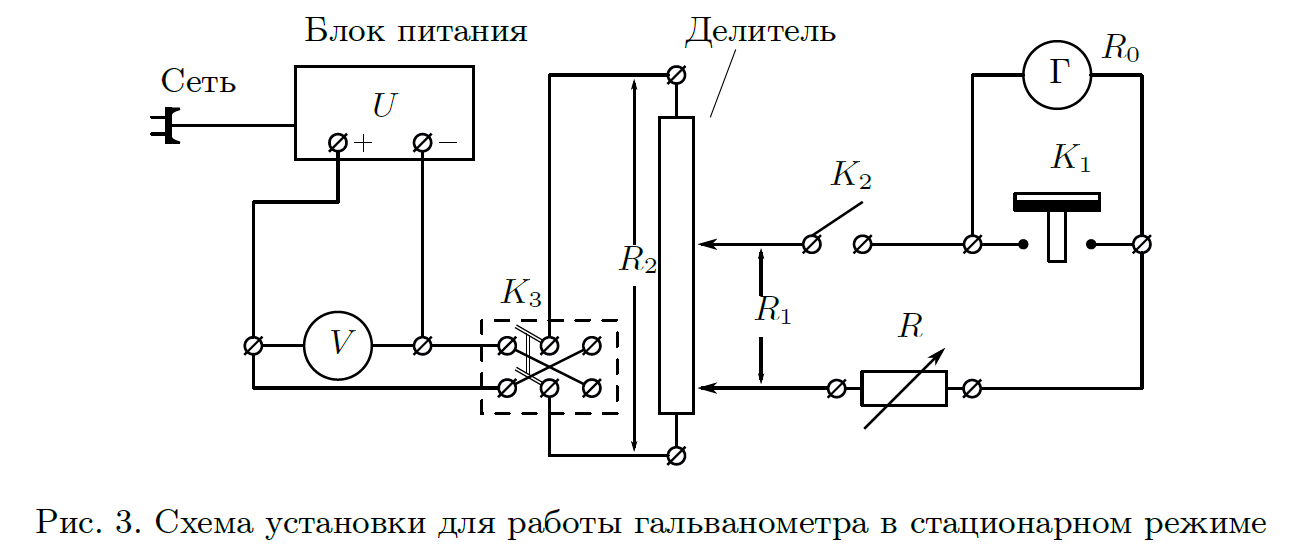
\includegraphics[width=1\textwidth]{уст1.png}
	\label{fig:boiler}
\end{figure}

Схема для исследования гальванометра в стационарном режиме представлена на рис. 3. Постоянное напряжение $U$ снимается с блока питания и измеряется вольтметром $V$. Ключ $K_3$ позволяет менять направление тока через гальванометр $\Gamma$, делитель напряжения - менять величину тока в широких пределах. Ключ $K_2$ служит для включения гальванометра, кнопка $K_1$ - для его успокоения. Магазин сопротивлений $R$ позволяет менять режим работы гальванометра от колебательного до апериодического.

Рис. 3. Схема установки для работы гальванометра в стационарном режиме

При $R_1 \ll R, R_0, R_2$ сила тока, протекающего через гальванометр, может быть вычислена как
$$
I=\frac{R_1}{R_2} \frac{U_0}{R+R_0},
$$

где $U_0$ - показания вольтметра, $R_1 / R_2$ - положение делителя, $R-$ coпротивление магазина, $R_0$ - внутреннее сопротивление гальванометра.

Угол отклонения рамки от положения равновесия измеряется с помощью осветителя, зеркальца, укреплённого на рамке, и шкалы, на которую отбрасывается луч света от зеркальца. Координата $x$ светового пятна на шкале связана с углом $\varphi$ отклонения рамки формулой
$$
x=a \operatorname{arctg} 2 \varphi,
$$

где $a$ - расстояние от шкалы до зеркальца. При малых углах можно считать, что $\varphi=x / 2 a$. Динамическую постоянную
$$
C_I=\frac{I}{\varphi}=\frac{2 a I}{x},
$$

как правило, выражают в единицах $\left[\frac{\mathrm{A}}{\text { мм/м }}\right]$ (ток $I$ измеряется в амперах, $x$ - в миллиметрах, $a-$ в метрах).

\subsection{Б. Определение критического сопротивления гальванометра}

Критическим сопротивлением баллистического гальванометра называется сопротивление его электрической цепи $R_{\text {кр }}$, при котором после начального толчка подвижная система почти экспоненциально возвращается к нулю, подчиняясь уравнению (17). На практике критический режим, требующий строгого выполнения условия $\gamma=\omega_0$, не может быть точно реализован и имеет значение как пограничный между режимом затухающих колебаний $\left(\gamma<\omega_0\right)$ и режимом апериодического затухания $\left(\gamma>\omega_0\right)$.

Измерение критического сопротивления гальванометра можно выполнить с помощью той же схемы (рис. 3).

При больших $R$ свободное движение рамки имеет колебательный характер. С уменьшением $R$ затухание увеличивается (см. (5), (10)), и колебательный режим переходит в апериодический.

В качестве характеристики процесса затухания колебаний рамки гальванометра воспользуемся представленным формулой (2.24) логарифмическим декрементом затухания:
$$
\Theta=\gamma T_1=\ln \frac{x_n}{x_{n+1}}
$$

где $x_n$ и $x_{n+1}$ - два последовательные отклонения колеблющейся величины в одну сторону. Измеряя зависимость $\Theta(R)$ логарифмического декремента затухания от сопротивления внешней цепи $R$, можно найти критическое сопротивление $R_{\text {кр }}$ как параметр зависимости, которая следует из выражений (15), (17) и (26):
$$
R_{\mathrm{Kp}}=\frac{R+R_0}{\sqrt{\left(\frac{2 \pi}{\Theta}\right)^2+1}}-R_0,
$$
или
$$
\sqrt{\frac{4 \pi^2}{\Theta^2}+1}=\frac{R+R_0}{R_{\text {кр }}+R_0}
$$

\subsection{В. Определение баллистической постоянной и критического сопротивления гальванометра, работающего в баллистическом режиме}

\begin{figure}[!h]
	\centering
	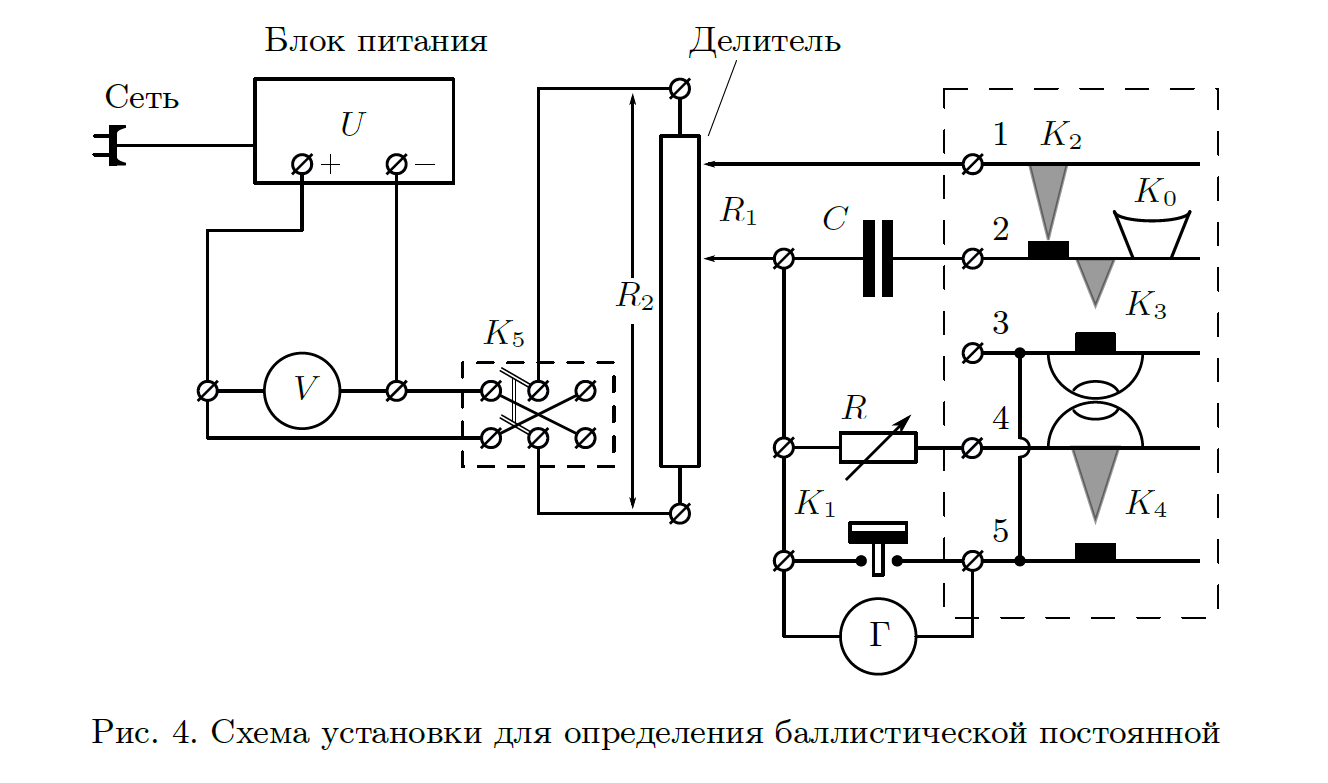
\includegraphics[width=1\textwidth]{уст2.png}
	\label{fig:boiler}
\end{figure}

Для изучения работы гальванометра в режиме измерения заряда (в баллистическом режиме), используется схема, представленная на рис. 4 .

Система ключей устроена так, что нормально ключ $K_2$ замкнут, а ключи $K_3$ и $K_4$ разомкнуты. При нажатии на кнопку $K_0$ сначала размыкается ключ $K_2$, затем замыкается $K_3$ и через некоторое время $-K_4$. При нормальном положении кнопки $K_0$ конденсатор $C$ заряжается до напряжения $U_C$ и получает заряд $q$ :
$$
U_C=\frac{R_1}{R_2} U_0, \quad q=C U_C=\frac{R_1}{R_2} U_0 C .
$$

При нажатии на ключ $K_0$ конденсатор отключается от источника постоянного напряжения (размыкается ключ $K_2$ ) и подключается к гальванометру (замыкается ключ $K_3$ ).
Рис. 4. Схема установки для определения баллистической постоянной
Ёмкость конденсатора выбрана так, что к моменту замыкания ключа $K_4$ весь заряд успевает пройти через гальванометр, и рамка получает начальную скорость $\dot{\varphi}(\tau)$ (см. (21)). При этом можно считать, что отклонение рамки, происходящее за время, протекающее между замыканием ключей $K_3$ и $K_4$, равно нулю. При замыкании ключа $K_4$ гальванометр шунтируется внешним сопротивлением $R$, и в зависимости от величины этого сопротивления движение рамки описывается одним из уравнений: (14), (16), (18) или (19).

Первый отброс зайчика $\varphi_{\max }$ после нажатия на кнопку $K_0$ зависит от сопротивления внешней цепи, подключённой к гальванометру. Для определения $R_{\text {кр }}$ используется то обстоятельство, что в критическом режиме максимальное отклонение зайчика в $e$ раз меньше, чем у гальванометра без затухания (см. (20) и (21)).

Следует помнить, что наблюдать колебания рамки при полном отсутствии затухания, конечно, невозможно, так как даже при разомкнутой внешней цепи $(R=\infty)$ остаётся трение в подвеске и трение рамки о воздух. Величину максимального отклонения рамки гальванометра без затухания $\varphi_{\max }^{\mathrm{cB}}$ можно, однако, рассчитать, если при разомкнутой цепи измерить реальное максимальное отклонение рамки $\varphi_0$ и логарифмический декремент затухания $\Theta_0$ (при $R=\infty$ величина $\Theta_0$ определяется только внутренним трением в рамке). Из уравнений (14) и (26) при $\gamma \ll \omega_0$ вытекают равенства
$$
\varphi_0=\varphi\left(T_1 / 4\right)=\varphi_{\max }^{\mathrm{cB}} e^{-\Theta_0 / 4},
$$

так что максимальное отклонение рамки гальванометра без затухания
$$
\varphi_{\max }^{\mathrm{cB}}=\varphi_0 e^{\Theta_0 / 4} \approx \varphi_0\left(1+\frac{\Theta_0}{4}\right) .
$$

Баллистическая постоянная гальванометра $C_q^{\text {кр }}\left[\frac{\text { Кл }}{\text { мм/м }}\right]$ определяется при критическом сопротивлении $\left(R=R_{\text {кр }}\right)$ :
$$
C_q^{\mathrm{KP}}=\frac{q}{\varphi_{\max }^{\mathrm{Kp}}}=2 a \frac{R_1}{R_2} \frac{C U_0}{x_{\max }^{\mathrm{Kp}}}
$$

где $x_{\max }^{\mathrm{\kappa p}}-$ величина первого отброса в критическом режиме, выраженная в делениях шкалы (мм), $a$ - расстояние от зеркальца до шкалы, выраженное в метрах, произведение $C U_0$ - заряд, выраженный в кулонах.

\section{Измерения, Обработка}

\subsection{I. Подготовка приборов к работе}

1) Подготовим прибор к работе, убедимся в корректной калибровку нуля

2) Установим делитель на отношение $\frac{R_1}{R_2} \approx \frac{1}{2000}$, а сопротивление магазина $R \approx 50$ кОм.

3) Соберем электрическую схему, плотно зажав контакты

4-5) Запустим схему, убедимся в корректности работы

6) Зайчик отклоняется почти на всю шкалу при $R = 5$ кОм.

\subsection{II. Определение динамической постоянной}

7) Результаты занесены в электронную таблицу

Показания вольтметра $U_0 = 1.36$ В

Положение делителя $\frac{R_1}{R_2} \approx \frac{1}{2000}$

Величина $R_2 = 10$ кОм

Сопротивление гальванометра $R_0 = 560$ Ом

\subsection{III. Определение критического сопротивления}

8 - 9) Два последовательных отклонения $x_1 = 23.7$ см, а $x_2 = 18.6$ см.

10) Период свободных колебаний измерю по последовательным 7 колебаниям

$7 T_0 = 33.74 \pm 0.14$ сек; $T_0 = 4.82 \pm 0.02$ сек.

11-12) Критическое сопротивление составило $R_\text{кр} = 7.7 \pm 0.1$ кОм.

13) Отношение делителя для полного заполнения шкалы составит $\frac{R_1}{R_2} \approx \frac{1}{500}$

14) Результаты занесем в таблицу.

\subsection{IV. Баллистический режим}

15) Соберем схему и запустим её

16-17) Занесем результаты измерений в таблицу.

18) Положение делителя $\frac{R_1}{R_2} \approx \frac{1}{50}$

Емкость $C = 2$ мкФ

Расстояние базы $a = 90$ см.

19) Разберем схему

\subsection{V. Обработка результатов}

\subsubsection{Динамическая постоянная}

20) Считая $I = U_0 \frac{R_1}{R_2}\frac{1}{R + R_0}$, построим график зависимости $I(x)$

\begin{figure}[!h]
	\centering
	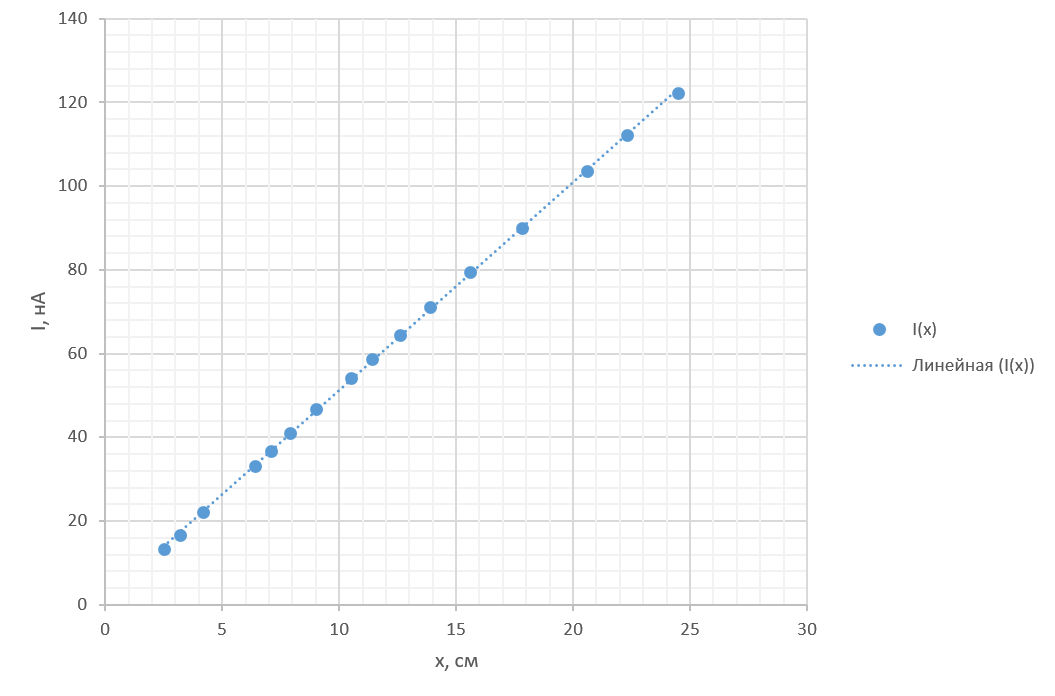
\includegraphics[width=1\textwidth]{граф1.png}
	\label{fig:boiler}
\end{figure}

Найдем угловые коэффициенты прямых для каждой установки по МНК.

\[
	a = \frac{<x_i y_i> - < x > < y_i >}{< x_i^2> - < x_i >^2}
\]

\[
	b = < \nu_i > - a < N_i >
\]

Также рассчитаем их погрешности

\begin{equation}
	S_a^2 = \frac{< x_i^2>}{< x_i^2 > - < x_i >^2} \cdot \frac{<  b_i - b > ^2}{n - 2}
\end{equation}

Итого линеаризация

\begin{equation}
	y = (a \pm Sa) + (b \pm Sb) \cdot x = (1.57 \pm 0.25) + (4.965 \pm 0.018) \pm x
\end{equation}

Визуально шкала линейная. Линеаризация это подтверждает. Однако используя переход к углам через $	atan \left( \frac{x}{a} \right)$ можно добиться истинно линейной шкалы.

Переходя к тангенсу угла, получим

\begin{equation}
	C_1 = 2 a tg \alpha = 2 a \cdot k = (8.94 \pm 0.09) \cdot 10^{-7} \text{ А} = (8.94 \pm 0.09) \cdot 10^{-4} \frac{\text{ А}}{\text{ мм/м}}
\end{equation}

Чувствительность гальванометра

\begin{equation}
	S_1 = \frac{1}{C_1} = (1.119 \pm 0.011) \cdot 10^{3} \frac{\text{ мм/м}}{\text{ А}}
\end{equation}

\subsubsection{Критическое сопротивление}

21) Логарифмический декремент затухания (значения отклонений усреднены)

$$
\Theta=\ln \frac{x_n}{x_{n+1}} = \ln \frac{23.7}{18.6} = 0.24 \pm 0.01
$$

22) Используя формулу для $R_\text{кр} = \frac{R+R_0}{1+\frac{4\pi^2}{\Theta^2}} - R_0 = const$, получим таблицу


.

\begin{table}[h]
	\centering
	\begin{tabular}{|c|c|c|c|c|c|}
		\hline
		$ N $& $ R, \; кОм $& $ x_n, $ см &$ x_{n+1}, $ см & $ \Theta $ & $ R_{\text{кр}} $, кОм\\
		\hline
		1 & 24 & 5.9 & 0.8 & 2.00 & 6.89 \\
		2 & 28 & 11.1 & 1.7 & 1.88 & 7.62 \\
		3 & 32 & 10.6 & 1.6 & 1.67 & 7.81 \\
		4 & 36 & 10.3 & 2.4 & 1.46 & 7.70 \\
		5 & 40 & 10.2 & 2.7 & 1.33 & 7.84 \\
		6 & 44 & 9.8 & 3.0 & 1.18 & 7.69 \\
		7 & 48 & 9.8 & 3.2 & 1.12 & 7.96 \\
		8 & 56 & 14.4 & 5.3 & 1.00 & 8.33 \\
		9 & 64 & 13.0 & 5.2 & 0.92 & 8.76 \\
		10 & 72 & 12.0 & 5.2 & 0.84 & 9.02 \\
		11 & 80 & 11.8 & 5.5 & 0.76 & 9.16 \\
		\hline
	\end{tabular}% 
	\label{resR}% 
\end{table}% 

Усреднив значения с 2 по 7 как наиболее повторяемые, получим результат  $ R_{\text{кр}} = 7.78 \pm 0.10 \; \text{ кОм} $

\subsubsection{Баллистическая постоянная}

23) Для холостого хода установки $l_x = 23.2$ см. Тогда $R\left( \frac{l_x}{e} \right) = R (8.53) = 7.5$ кОм. С учетом того, что $R = R_\text{кр} + R_0$, получим $R_\text{кр} \simeq 7$ кОм.

24-26) Баллистическая постоянная

\begin{equation}
	C_{Q_{\text{кр}}} = 2a \dfrac{R_1}{R_2} \dfrac{U_0C}{l_e} = 1.15 \cdot 10^{-6} \; \text{ Кл}
\end{equation}

Время релаксации $\tau = R_0 C \approx 1.1$ мс, что сильно меньше периода

\section{Вывод}

Значения $R_\text{кр}$ получились довольно близки (7.7, 7.78, 7) кОм, а время релаксации много меньше периода колебаний. Все это подчеркивает, что принятые электродинамические и механические приближения в этой задаче оправданны.

\section{Ресурсы}

Расчет по МНК: метод-наименьших-квадратов.рф


\end{problem}
\end{document}